% !TEX root = ../HonoursThesisTemplate.tex

\chapter{Ordinal Partitions}

    
`Ordinal analysis', first introduced by Bandt and Pompe (2002), proposed using the ordering of data points to partition a time series. Each data point in the timeseries is partitioned according to the ordering of its preceding points, and assigned a unique `ordinal symbol', for example numbers from 1 to 6.

The probabilities of the timeseries transitioning from one partition to another can be calculated, giving the `ordinal transition probabilities'.

\begin{figure}
    \centering
    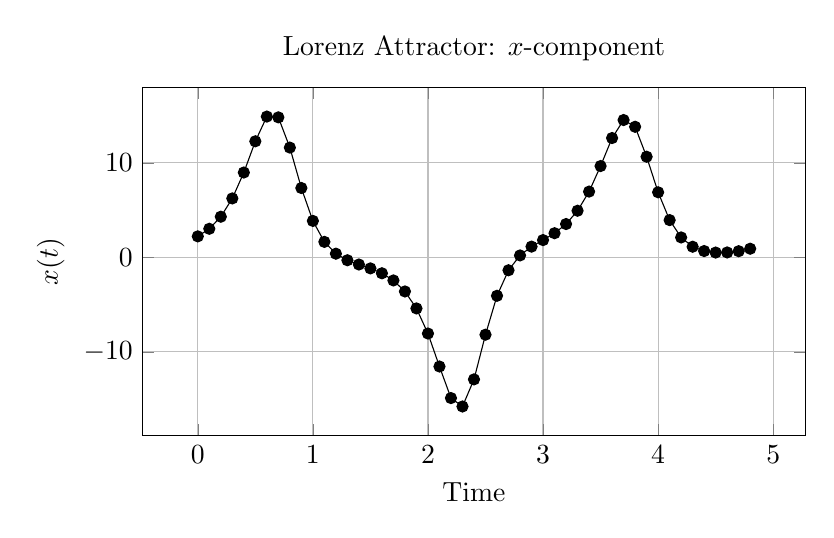
\begin{tikzpicture}
        \begin{axis}[
            xlabel={Time},
            ylabel={$x(t)$},
            title={Lorenz Attractor: $x$-component},
            width=10cm, height=6cm,
            grid=major
        ]
        % Data generated by solving dx/dt = sigma(y - x), etc. in Python
        \addplot[black, mark=*, mark options={black}] coordinates {
            (0.0, 2.2165566502619796)
            (0.1, 3.0181360987381685)
            (0.2, 4.2948078524935065)
            (0.3, 6.231121537780632)
            (0.4, 8.970926893912857)
            (0.5, 12.272230400810887)
            (0.6, 14.887997312478161)
            (0.7, 14.803117347063516)
            (0.8, 11.606868473299526)
            (0.9, 7.330990437181266)
            (1.0, 3.85191889651296)
            (1.1, 1.6347534154776406)
            (1.2, 0.3853895148599277)
            (1.3, -0.30838099414996695)
            (1.4, -0.7586726217449103)
            (1.5, -1.1695821908357407)
            (1.6, -1.6858338981790886)
            (1.7, -2.443141458426554)
            (1.8, -3.6086854451117074)
            (1.9, -5.40339197322587)
            (2.0, -8.058505977971057)
            (2.1, -11.547145254692042)
            (2.2, -14.884182443761347)
            (2.3, -15.775516623377253)
            (2.4, -12.908181797239536)
            (2.5, -8.181376578133673)
            (2.6, -4.06724026097539)
            (2.7, -1.3665393788429014)
            (2.8, 0.20110496364168012)
            (2.9, 1.1324784341364973)
            (3.0, 1.8245674314417792)
            (3.1, 2.5516132966355554)
            (3.2, 3.5214281335608555)
            (3.3, 4.926987945369609)
            (3.4, 6.951562500713474)
            (3.5, 9.654345729238477)
            (3.6, 12.617195234374243)
            (3.7, 14.521825487882024)
            (3.8, 13.806356286601272)
            (3.9, 10.64113968132102)
            (4.0, 6.880279139891668)
            (4.1, 3.9367704788159394)
            (4.2, 2.1029851064946445)
            (4.3, 1.121305395878461)
            (4.4, 0.665491176850325)
            (4.5, 0.5051437108082056)
            (4.6, 0.5156168027361644)
            (4.7, 0.6490783162490397)
            (4.8, 0.9105168761220792)
        };
        \end{axis}
    \end{tikzpicture}
    \caption{This is the caption}
    \label{fig:label}
\end{figure}

\begin{figure}
    \begin{center}
        \begin{tikzpicture}[scale=0.95]
            % partition 1

            \node[circle, draw, fill=col1] (topleft) at (-5.0, 3) {};

            % Draw the equality sign
            \node at (-4.6, 3) {$=$};
            
            % Draw the nodes in the lower part
            \node[circle, draw] (1_2) at (-4.0, 4) {1};
            \node[circle, draw] (1_1) at (-3.25, 3) {2};
            \node[circle, draw, thick, fill=col1] (1_3) at (-2.5, 2) {3};
            
            % Draw edges
            \draw (1_1) -- (1_2);
            \draw (1_1) -- (1_3);

            % Draw dividing line
            \draw[gray, very thin] (-1.6, 5) -- (-1.6, -3);

            % partition 2

            \node[circle, draw, fill=col2] (topcentre) at (-1, 3) {};

            % Draw the equality sign
            \node at (-0.6, 3) {$=$};
            
            % Draw the nodes in the lower part
            \node[circle, draw] (2_2) at (0, 4) {1};
            \node[circle, draw] (2_1) at (0.75, 2) {3};
            \node[circle, draw, thick, fill=col2] (2_3) at (1.5, 3) {2};
            
            % Draw edges
            \draw (2_1) -- (2_2);
            \draw (2_1) -- (2_3);

            % Draw dividing line
            \draw[gray, very thin] (2.5, 5) -- (2.5, -3);

            % partition 3

            \node[circle, draw, fill=col3] (topleft) at (3.0, 3) {};

            % Draw the equality sign
            \node at (3.4, 3) {$=$};
            
            % Draw the nodes in the lower part
            \node[circle, draw] (3_2) at (4.0, 3) {2};
            \node[circle, draw] (3_1) at (4.75, 4) {1};
            \node[circle, draw, thick, fill=col3] (3_3) at (5.5, 2) {3};
            
            % Draw edges
            \draw (3_1) -- (3_2);
            \draw (3_1) -- (3_3);

            % Draw dividing line
            \draw[gray, very thin] (-5, 1) -- (6, 1);

            % partition 4

            \node[circle, draw, fill=col4] (bottomleft) at (-5.0, -1.5) {};

            % Draw the equality sign
            \node at (-4.6, -1.5) {$=$};
            
            % Draw the nodes in the lower part
            \node[circle, draw] (4_2) at (-4.0, -1.5) {2};
            \node[circle, draw] (4_1) at (-3.25, -2.5) {3};
            \node[circle, draw, thick, fill=col4] (4_3) at (-2.5, -0.5) {1};
            
            % Draw edges
            \draw (4_1) -- (4_2);
            \draw (4_1) -- (4_3);

            % Draw dividing line
            % \draw[gray, very thin] (-2.25, -3) -- (-2.25, -5);

            % partition 5

            \node[circle, draw, fill=col5] (bottomcentre) at (-1, -1.5) {};

            % Draw the equality sign
            \node at (-0.6, -1.5) {$=$};
            
            % Draw the nodes in the lower part
            \node[circle, draw] (5_2) at (0, -2.5) {3};
            \node[circle, draw] (5_1) at (0.75, -1.5) {2};
            \node[circle, draw, thick, fill=col5] (5_3) at (1.5, -0.5) {1};
            
            % Draw edges
            \draw (5_1) -- (5_2);
            \draw (5_1) -- (5_3);

            % partition 6

            \node[circle, draw, fill=col6] (bottomright) at (3.0, -1.5) {};

            % Draw the equality sign
            \node at (3.4, -1.5) {$=$};
            
            % Draw the nodes in the lower part
            \node[circle, draw] (6_2) at (4.0, -2.5) {3};
            \node[circle, draw] (6_1) at (4.75, -0.5) {1};
            \node[circle, draw, thick, fill=col6] (6_3) at (5.5, -1.5) {2};
            
            % Draw edges
            \draw (6_1) -- (6_2);
            \draw (6_1) -- (6_3);
        \end{tikzpicture}
    \end{center}
    \caption{this is the caption}
    \label{fig:labelhere}
\end{figure}

\begin{figure}
    \centering
    \begin{tikzpicture}
    \begin{axis}[
        xlabel={Time},
        ylabel={$x(t)$},
        title={Lorenz Attractor: $x$-component},
        width=10cm, height=6cm,
        grid=major
    ]


    \addplot [
        thick, % or any style you like
    ] coordinates {
        (0.0, 2.2165566502619796)
        (0.1, 3.0181360987381685)
        (0.2, 4.2948078524935065)
        (0.3, 6.231121537780632)
        (0.4, 8.970926893912857)
        (0.5, 12.272230400810887)
        (0.6, 14.887997312478161)
        (0.7, 14.803117347063516)
        (0.8, 11.606868473299526)
        (0.9, 7.330990437181266)
        (1.0, 3.85191889651296)
        (1.1, 1.6347534154776406)
        (1.2, 0.3853895148599277)
        (1.3, -0.30838099414996695)
        (1.4, -0.7586726217449103)
        (1.5, -1.1695821908357407)
        (1.6, -1.6858338981790886)
        (1.7, -2.443141458426554)
        (1.8, -3.6086854451117074)
        (1.9, -5.40339197322587)
        (2.0, -8.058505977971057)
        (2.1, -11.547145254692042)
        (2.2, -14.884182443761347)
        (2.3, -15.775516623377253)
        (2.4, -12.908181797239536)
        (2.5, -8.181376578133673)
        (2.6, -4.06724026097539)
        (2.7, -1.3665393788429014)
        (2.8, 0.20110496364168012)
        (2.9, 1.1324784341364973)
        (3.0, 1.8245674314417792)
        (3.1, 2.5516132966355554)
        (3.2, 3.5214281335608555)
        (3.3, 4.926987945369609)
        (3.4, 6.951562500713474)
        (3.5, 9.654345729238477)
        (3.6, 12.617195234374243)
        (3.7, 14.521825487882024)
        (3.8, 13.806356286601272)
        (3.9, 10.64113968132102)
        (4.0, 6.880279139891668)
        (4.1, 3.9367704788159394)
        (4.2, 2.1029851064946445)
        (4.3, 1.121305395878461)
        (4.4, 0.665491176850325)
        (4.5, 0.5051437108082056)
        (4.6, 0.5156168027361644)
        (4.7, 0.6490783162490397)
        (4.8, 0.9105168761220792)
    };
    
    
    % Define how each "class" (symbolic label) is colored and drawn:
    \addplot[
        scatter,
        only marks,
        scatter src=explicit symbolic,
        scatter/classes={
            1={mark=*,draw=col1,fill=col1},
            2={mark=*,draw=col2,fill=col2},
            3={mark=*,draw=col3,fill=col3},
            4={mark=*,draw=col4,fill=col4},
            5={mark=*,draw=col5,fill=col5},
            6={mark=*,draw=col6,fill=col6}
        }
    ] 
    coordinates {
        (0.0, 2.2165566502619796)[2]
        (0.1, 3.0181360987381685)[5]
        (0.2, 4.2948078524935065)[5]
        (0.3, 6.231121537780632)[5]
        (0.4, 8.970926893912857)[5]
        (0.5, 12.272230400810887)[5]
        (0.6, 14.887997312478161)[5]
        (0.7, 14.803117347063516)[6]
        (0.8, 11.606868473299526)[1]
        (0.9, 7.330990437181266)[1]
        (1.0, 3.85191889651296)[1]
        (1.1, 1.6347534154776406)[1]
        (1.2, 0.3853895148599277)[1]
        (1.3, -0.30838099414996695)[1]
        (1.4, -0.7586726217449103)[1]
        (1.5, -1.1695821908357407)[1]
        (1.6, -1.6858338981790886)[1]
        (1.7, -2.443141458426554)[1]
        (1.8, -3.6086854451117074)[1]
        (1.9, -5.40339197322587)[1]
        (2.0, -8.058505977971057)[1]
        (2.1, -11.547145254692042)[1]
        (2.2, -14.884182443761347)[1]
        (2.3, -15.775516623377253)[1]
        (2.4, -12.908181797239536)[4]
        (2.5, -8.181376578133673)[5]
        (2.6, -4.06724026097539)[5]
        (2.7, -1.3665393788429014)[5]
        (2.8, 0.20110496364168012)[5]
        (2.9, 1.1324784341364973)[5]
        (3.0, 1.8245674314417792)[5]
        (3.1, 2.5516132966355554)[5]
        (3.2, 3.5214281335608555)[5]
        (3.3, 4.926987945369609)[5]
        (3.4, 6.951562500713474)[5]
        (3.5, 9.654345729238477)[5]
        (3.6, 12.617195234374243)[5]
        (3.7, 14.521825487882024)[5]
        (3.8, 13.806356286601272)[6]
        (3.9, 10.64113968132102)[1]
        (4.0, 6.880279139891668)[1]
        (4.1, 3.9367704788159394)[1]
        (4.2, 2.1029851064946445)[1]
        (4.3, 1.121305395878461)[1]
        (4.4, 0.665491176850325)[1]
        (4.5, 0.5051437108082056)[1]
        (4.6, 0.5156168027361644)[2]
        (4.7, 0.6490783162490397)[5]
        (4.8, 0.9105168761220792)[5]
    };
    
    \end{axis}
    \end{tikzpicture}
    \caption{this is the caption}
    \label{fig:labelhere}
\end{figure}

\begin{table}[]
    \centering
    \begin{tabular}{c|cccccc}
        & \tikz\draw[fill=col1,draw=col1] (0,0) circle (0.9ex); 
        & \tikz\draw[fill=col2,draw=col2] (0,0) circle (0.9ex); 
        & \tikz\draw[fill=col3,draw=col3] (0,0) circle (0.9ex); 
        & \tikz\draw[fill=col4,draw=col4] (0,0) circle (0.9ex); 
        & \tikz\draw[fill=col5,draw=col5] (0,0) circle (0.9ex); 
        & \tikz\draw[fill=col6,draw=col6] (0,0) circle (0.9ex); \\ \hline
        \tikz\draw[fill=col1,draw=col1] (0,0) circle (0.9ex); & 0.7 & 0.1 & 0.1 & 0.05 & 0.05 & 0.0 \\
        \tikz\draw[fill=col2,draw=col2] (0,0) circle (0.9ex); & 0.0 & 0.0 & 0.0 & 0.0 & 0.9 & 0.1 \\
        \tikz\draw[fill=col3,draw=col3] (0,0) circle (0.9ex); & 0.7 & 0.1 & 0.1 & 0.05 & 0.05 & 0.0 \\
        \tikz\draw[fill=col4,draw=col4] (0,0) circle (0.9ex); & 0.0 & 0.0 & 0.0 & 0.0 & 0.9 & 0.1 \\
        \tikz\draw[fill=col5,draw=col5] (0,0) circle (0.9ex); & 0.0 & 0.0 & 0.0 & 0.0 & 0.9 & 0.1 \\
        \tikz\draw[fill=col6,draw=col6] (0,0) circle (0.9ex); & 0.7 & 0.05 & 0.05 & 0.05 & 0.05 & 0.1 \\
    \end{tabular}
    \caption{Transition probabilities between ordinal partitions.}
    \label{tab:transition_probabilities}
\end{table}
